\section{A Big Pitfall: What If You Suddenly Lose All Your Computer Data Tomorrow? — How to Back Up Your Files}

\begin{figure}[H]
    \begin{tabular}{rl}
        
\includegraphics[width=0.5\columnwidth]{author-folder/Kai.Wu/backup1.jpg} &
        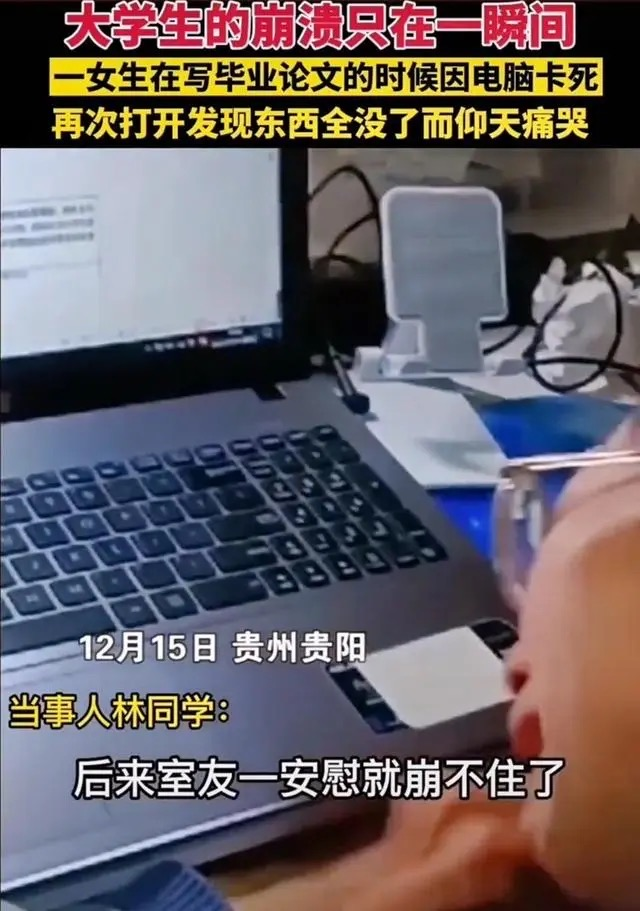
\includegraphics[width=0.4\columnwidth]{author-folder/Kai.Wu/backup2.jpg}
    \end{tabular}
    \caption{\href{https://baijiahao.baidu.com/s?id=1719578217211021768}{Link: A Female University Student in Guiyang Lost Her 8,000-Word Graduation Thesis and Broke Down Crying}}
\end{figure}

Most students buy their own computers during their undergraduate years. Although all their assignments, research data up to the PhD stage, and papers are stored only on this one computer, they are not fully aware of the importance of their computer and the fragility of the information stored on it. Every year, incidents like the one shown above occur, causing heavy blows to those involved, such as making news headlines and being ridiculed nationwide.

Losing a paper you're working on is actually a small matter since all the research data is still there. The person in the news above rewrote the paper in just a few days. But are those extremely important yet seldom-accessed materials absolutely safe?

Imagine if:
\begin{itemize}
    \item One day, your hand slips, the computer falls to the ground, won't boot anymore, and the hard drive can't be recovered.
    \item On a groggy day, you grab a cup of coffee and accidentally spill it on your computer, causing an instant short circuit with sizzling sounds.
    \item You unwittingly click on a link and get infected with ransomware; or the XJTLU intranet is attacked, and all computers are infected with ransomware. All your files are encrypted and locked.
    \item You take your computer out for work or data collection, and the entire computer gets stolen.
    \item On your way home for the holidays, your backpack or suitcase gets stolen or taken by mistake.
    \item Without any malice, but what if XJTLU catches fire, gets flooded (the 5th floor of MB leaks during heavy rain), or the building collapses, and you don't have time to grab your computer during evacuation.
\end{itemize}

\begin{figure}[H]
    \centering
    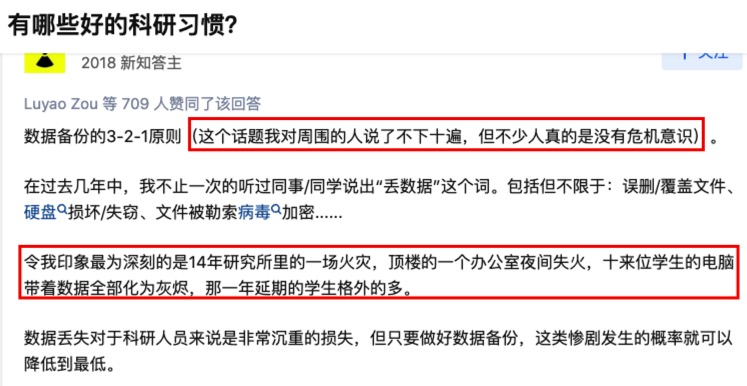
\includegraphics[width=0.8\columnwidth]{author-folder/Kai.Wu/backup_zhihu.jpg}
    \caption{\url{https://www.zhihu.com/question/394796969/answer/1501840215}}
\end{figure}

Individually, these situations are rare, but adding up all the possibilities over three to four years, the probability of at least one occurring is not small. If it happens, how much will your PhD progress be delayed, and how much of your youth will be wasted?

Having only one copy of your data is extremely fragile. Think now: are the computers, data, and papers you rely on stored only in one place? If so, please get up from your chair immediately, go to the bathroom and wash your face, ask yourself how you can be so careless as an adult, and then start reading the guide below.

\subsection{Theory: The 3-2-1 Principle}

The "3-2-1 Principle" is a common data backup method used by commercial companies, specifically:
\begin{itemize}
    \item 3: Keep 3 complete copies of your files—one original and two backups.
    \item 2: Store the files on at least two different types of media.
    \item 1: Keep one backup copy off-site.
\end{itemize}

The "media" refers to different storage mediums such as internal hard drives, external hard drives, USB drives, cloud drives, etc. It may sound complicated, but the simplest practice for us is: keep the original on the internal hard drive, and store two backups on an external hard drive and a cloud drive respectively, thus meeting all three requirements simultaneously. This way, you can handle all the catastrophic problems listed above (even if the cloud drive company suddenly goes bankrupt) without affecting your research.

\subsection{Practice}

Now it's time to get started. First, decide the scope of your backup based on your resources. In the most extravagant scenario, you can make a local backup of your entire computer plus a cloud drive backup. However, often the cloud storage space is limited, external hard drive capacity may be insufficient, or the network speed is too slow to upload too much data. So, first define the scope of your backup.

\begin{itemize}
    \item The most economical solution: Only back up the most important files, such as papers, research data, CV, and desktop. Use real-time cloud backup + periodic external hard drive backup. This requires very little capacity on both the external hard drive and cloud drive.
    \item The most efficient solution: Locally back up the entire computer (including the most important data); add one more real-time cloud backup for the most important research papers, etc. This requires an external hard drive larger than your computer's hard drive (not expensive), plus a normal capacity (about 10 GB) cloud drive.
    \item \sout{The most extravagant solution: Buy a NAS, insert several tens of terabytes of drives, set up RAID 1, and then synchronously transfer a copy to an off-site location.}
\end{itemize}

A typical computer hard drive capacity is generally within 2 TB. I assume it's not too much to ask for everyone to buy an external hard drive of 2 TB or more (within 500 yuan). If your supervisor has sufficient funding, you can directly ask for one—just say you want an external hard drive for backup and see if they can help you purchase one. Reimbursements within 2,000 yuan are quite easy. Therefore, I'll only introduce the efficient method below.

\subsubsection{Full Computer Backup}
\label{sec.pc_backup}

One major benefit of making a full backup of your computer is that if your computer is completely lost, you can fully restore your previous working state within one day after buying a new computer, seamlessly resuming your work without affecting your research.

Windows and macOS both come with built-in system-level full backup solutions. There are many tutorials online, so I won't elaborate.

\begin{itemize}
    \item For Windows, search "Windows backup" on Bilibili for tutorials. Generally, use the system's "Backup and Restore (Windows 7)" (although it says Windows 7, it works perfectly on Windows 10 and Windows 11, which is why it hasn't been discarded). For example, watch this video: \url{https://www.bilibili.com/video/BV1Dy4y1x7RP}
    \item For macOS, search "Mac Time Machine" on Bilibili. Generally, use "Time Machine" in System Settings. For example, watch this video: \url{https://www.bilibili.com/video/BV1oy4y177qS}
\end{itemize}

If one video isn't clear, don't worry—search for a few more to watch, and also make good use of Google and Zhihu. Beginners may feel that the learning cost is a bit high, but don't wait until your computer crashes to start preparing.

\subsubsection{Cloud Drive Backup}
\label{sec.net_drive_backup}

Box (\url{https://box.xjtlu.edu.cn/}) is the school's self-built cloud drive, upgraded in 2022 to provide 100 GB of free space per person. Upload and download speeds within the intranet can reach gigabit levels, and it comes with three months of file history versions, outperforming many other cloud drives. Drag important folders into the Seafile client (without moving folders), and it will automatically back up to the school's cloud drive in real time. Usage instructions can be found at \url{https://guide.xjtlu.edu.cn/box/student/drive_client/drive_clent_for_windows.html}. The only problem with Box is that it does not support file-sharing links (teachers have sharing permissions; students do not), but it's very suitable as a backup cloud drive.

Additionally, if you don't fully trust the school's IT, you can also install another commercial cloud drive for a second layer of cloud backup. I personally strongly do not recommend Baidu Cloud because it occasionally loses files randomly. Among domestic cloud drives, I recommend Nutstore (free version has unlimited space but limits monthly traffic). For foreign cloud drives, I recommend OneDrive (5 GB free for personal accounts; you can search on Taobao to expand OneDrive storage to 15 GB permanently for a few yuan). Additionally, everyone has a free 1 TB of OneDrive storage under their Liverpool account—take advantage of it (but remember to migrate your data before graduation because the account will be reclaimed). Refer to this section \ref{sec.fuli_liverpool}.

\subsection{Paper Backup and File History Versions}
\begin{minipage}[t]{0.65\textwidth}
    The backup methods mentioned above can handle most data loss scenarios. However, your papers, including dissertations and journal articles—the most important yet fragile materials—not only fear loss but also especially fear these two devastating disasters:
    \begin{enumerate}
        \item Version confusion. It's common to modify a paper dozens of times from the beginning to completion. Especially when nearing submission, you'll inevitably battle through a dozen more versions due to feedback from your supervisor, co-supervisor, and collaborators. The differences between versions may be minimal and hard to distinguish. There will inevitably come a day when you can't figure out which version is which or forget what modifications were made in which version, leading to repeated time spent distinguishing versions, which in turn leads to ↓
        \item File overwriting, such as (1) a new version directly overwriting the old version, but after a while, you need to retrieve the old version for some reason; (2) the old version overwriting the new one, wasting months of revisions.
    \end{enumerate}
\end{minipage}
\begin{minipage}[t]{0.34\textwidth}
    \begin{figure}[H]
        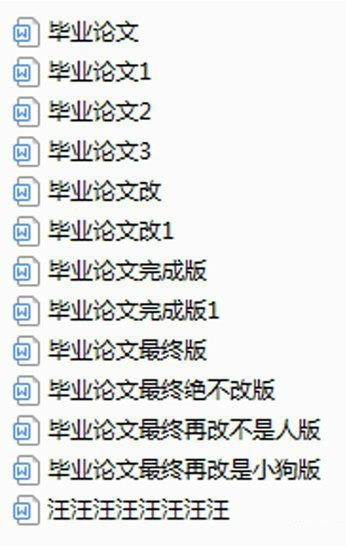
\includegraphics[width=0.95\columnwidth, right]{author-folder/Kai.Wu/thesis_versions.jpg}
    \end{figure}
\end{minipage}

At this point, if you're interested, you can do an experiment: create a file and write some content in it. Then, in another folder, create a file with the same name and write different content. Finally, drag it over to overwrite the previous file. Now, see if you have any way to retrieve the content of the previous file.

You might ask, didn't we mention so many backup methods above? Yes, but those backup methods mainly serve to prevent loss, like the computer being lost or hard drive failure, but few backups can prevent overwriting. For example, real-time backup cloud drives: if you mistakenly overwrite the file locally, it will be immediately overwritten in the cloud as well. Local backup hard drives: if the backup frequency isn't high, there's still a chance, but if you look for it after a while, you might not find it.

Therefore, for the safety of your paper (your lifeline), it's entirely worth adding another layer of insurance:

\begin{enumerate}
    \item Enable system-level File History protection in Windows: \url{https://www.asus.com.cn/support/FAQ/1013067/}. Don't forget to add your paper folder to make it effective.
    \item macOS's Time Machine backups come with a file history function. Refer to the previous section \ref{sec.pc_backup} to configure Time Machine, and the file history of your entire computer will be included in the backup.
    \item Linux users, I'm sure you have your methods. The simplest way is to write a shell script that directly copies the paper folder to another directory, naming it with the date. Finally, add this script to crontab to run periodically.
    \item The above are methods to enable local file history. Some cloud drives come with file versioning functions but usually limit the number or dates of versions or require a membership purchase to enable file versions. After enabling them, it's equivalent to also storing a version history in the cloud. In case your local settings aren't properly configured or can't be used for some reason, it can save you when you mistakenly overwrite files. The school's Seadrive comes with about two months of file versions, free and very generous. Again, I recommend everyone use it. Just drag the folder in to back up, and it will automatically generate file versions. See section \ref{sec.net_drive_backup}.
    \item For those who know a bit of Git and GitHub, please create a Git repository for your entire paper folder and upload it to GitHub as a private repo. Commit once every day after work to back up versions and record what content you modified. For papers, Git is the most perfect backup solution, allowing you to easily roll back to older versions without ever worrying about overwriting, and even easily know when a change was introduced, more reliable than all the above methods. Overleaf also has GitHub integration, making it convenient to collaborate with supervisors. But Git has a slightly higher learning cost, but there are countless detailed tutorials online. Interested and capable students can learn on their own.
\end{enumerate}

\begin{flushright}
    (December 2, 2022 by \Wu)

    (Major update: December 30,

    (major update: 2022年12月30日 by \Wu)

    Translated by GPT
\end{flushright}

% \begin{figure}[H]
%     \centering
%     \includegraphics[width=0.5\columnwidth]{author-folder/Kai.Wu/}
% \end{figure}


% \usepackage[export]{adjustbox}

% \item 
% \begin{minipage}{0.3\textwidth}
%     文字
% \end{minipage}
% \begin{minipage}{0.63\textwidth}
%     \begin{figure}[H]
%         \includegraphics[width=0.95\columnwidth, right]{author-folder/Kai.Wu/}
%     \end{figure}
% \end{minipage}

% \input{author-folder/Kai.Wu/.tex}
